\scanpage{12}

\textcircled{\unsure{10|9}°} Si $T$ noeth. \unsure{irred.} sur $S$, $\exists U\subset T$ ouvert non vide tel que $F_U$ soit représentable.
\margin{peut se formuler de façon un \unsure{peu plus} faible, avec impossibilité \unsure{générique} de prolonger}

\textcircled{1°} Foncteur $F$ de nature locale

\textcircled{2°} $F$ compatible avec descente fid plt qu. \unsure{cpte}
\margin{\uuline{localité}}

\textcircled{3°} $F$ commute aux $\varinjlim$ d'anneaux

\textcircled{4°} $F$ commute aux $\varprojlim$ d'anneaux \inserted{Artiniens} sous les conditions habituelles

\textcircled{\unsure{7|5}°} $F$ ``non ramifié'' \deleted{\unsure{et}} (Il suffit: sur les artiniens)
\inserted{et \unsure{$=$|m\textsuperscript{e}}: sur les $k[T]/(t^2)$}

\deleted{6° Tout pt de $F$ à valeurs dans une \deleted{corps} \inserted{extension} $K$ d'un $k(s)$, provient d'une sous-extension finie}

\textcircled{\unsure{5|7}°} $F$ proreprésentable universellement,
\figure{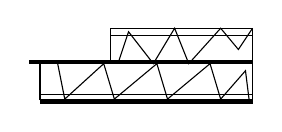
\begin{tikzpicture}[x=.45cm,y=.45cm]
\draw (0,0)--(6,0)--(6,2)--(2,2)--(2,1)--(0,1)--cycle;
\draw[line width=1.2pt] (-.3,1.05)--(6,1.05) (0,-.08)--(6,-.08);
\draw (0.5,1)--(.7,0)--(1.8,1)--(2.1,0)--(3.3,1)--(3.6,0)--(4.8,1)--(5.1,0)--(5.8,.8)--(5.9,0);
\draw (2.2,1)--(2.5,1.9)--(3.2,1)--(3.8,2)--(4.2,1)--(5.1,2)--(5.6,1.4)--(6,2);
\draw (0,.12)--(6,.12) (2,1.8)--(6,1.8);
\end{tikzpicture}}

\textcircled{8°}: $F$ ``séparé'' (critère valuatif).

\textcircled{9°} Pour tt $A$ anneau local noeth \inserted{complet} de dim 1, irréductible, sur $S$, et $\forall$ idéal $I$ de $A$ nilpotent, \inserted{i.e. $\unsure{\mathfrak p}$ idéal \unsure{premier|primaire}} \deleted{\unsure{$\xi$}} $\unsure{\xi_0|\eta_0}\in F(A/I)$, \deleted{\unsure{si $\unsure{\xi_0|\eta_0}\in\operatorname{Im}F(A_{\unsure{\mathfrak p|\eta}})$}} \deleted{\unsure{se prolonge en un $\unsure{\eta|y}\in F(A/\unsure{I^n})$,}} \deleted{\unsure{alors $\xi\in\varprojlim(A/\unsure{I^n})$}} \deleted{\unsure{provenant d'un} \illegible{1} \unsure{pour} $\xi_0\in F(A_{\unsure{\mathfrak p|\eta}}/I_{\unsure{\mathfrak p|\eta}})$}
\margin{automatique dans le cas étale}

\margin{\uline{9°} Pour $\forall S'$ \inserted{\unsure{noeth. irred.}} sur $S$, muni d'un \deleted{\unsure{schéma}} \inserted{Idéal} $I$ de carré nul [si on veut, \unsure{annulé par le nilradical}], définissant $S'_0=V(I)$, et $\forall\unsure{\eta|y}_0:\deleted{\unsure{S'_0}}\inserted{S'_0\to F_{S'}}$ ($S'$-linéaire), qui ne se prolonge pas au pt. gén. $\unsure{\eta|y}$ à un plus-\unsure{petit|grand} sous-schéma de $S'_{\unsure{\eta|y}}$ que $S'_{0\unsure{\eta|y}}$, il existe un voisinage ouvert $U$ de $\unsure{\eta|y}$, tel que pour tt $s\in S'$, $\unsure{\eta|y}|S'^s_0$ ne se prolonge pas à un plus grand sous-schéma de $S'^s$.
\diagram{\begin{tikzcd} F_{S'}\arrow[d,no head] & \\ S'\arrow[r,no head] & S'_0 \end{tikzcd}}
\deleted{\diagram{\begin{tikzcd} S' & \unsure{X}\arrow[l] \end{tikzcd}}}
\textcircled{A bis}}

\margin{N.B. \uline{8° et 9°} peuvent se remplacer par une condition unique, \unsure{faisant intervenir la|formulant la} \unsure{représentabilité} \unsure{non} dans la \unsure{formulation}, \unsure{en disant que une condition} \unsure{Modulaire ou} \unsure{pro-modulaire}, \deleted{$\unsure{F}$} \unsure{commute à l'extension} (\unsure{fid. plt}) de la base}

\margin{\deleted{peut se remplacer \uline{par}: si $A\to A'$ est injectif, $A'$ fini sur $A$, \deleted{\unsure{fid plt sur}} $A$ artinien \inserted{local}, \deleted{\unsure{alors $F(A)\xrightarrow{\sim}F(A')$}} [ext. résiduelle triviale, \deleted{\unsure{longueur}} $\operatorname{long}_A A'/A=1$] alors $F(A)\xrightarrow{\sim}F(A')$}}

\diagram{\begin{tikzcd}[column sep=large,row sep=large]
\unsure{7}^\circ\arrow[ddr,bend right=35] & \\
\text{peut se remplacer par}\arrow[r] & \unsure{5}^\circ \\
&9^\circ\arrow[dll,bend left=15]\\
\text{automatique dans le cas étale} &&
\end{tikzcd}}
\mspage{11}
